% textidote: ignore begin
\section{State of the Art}\label{sec:state-of-the-art}
% textidote: ignore end

The following section will look at and analyze existing solutions and their approach to visualizing statistics and
analytics, while looking for inspirations or areas to improve upon.
The chosen solutions are \acrlong{ga4} and Microsoft BI, as they are both widely used for commercial purposes and
provide a wide range of features.
% TODO change microsoft bi to a different analytics tool that could fit better for the solution

\subsection{Google Analytics}\label{subsec:google-analytics}

% textidote: ignore begin % textidote doesn't like it when sentences start with acronyms
\acrfull{ga4} is a general purpose analytics tool that can provide data on a wide arrange of services, such as websites,
online stores, and mobile applications~\cite{ga4}.
% textidote: ignore end
Its main highlights are the ability to track website views, store sales, user interactions, and much more data.
% textidote: ignore begin
\acrshort{ga4} is also highly customizable, allowing a manager to create custom fields and metrics, as well as custom
reports and dashboards.
% textidote: ignore end
The main purpose of \acrshort{ga4} is to help businesses with their marketing strategies, by providing data on user
behavior and demographics, as well as tracking the effectiveness of marketing campaigns.

% textidote: ignore begin
\begin{figure}[H]
    \centering
    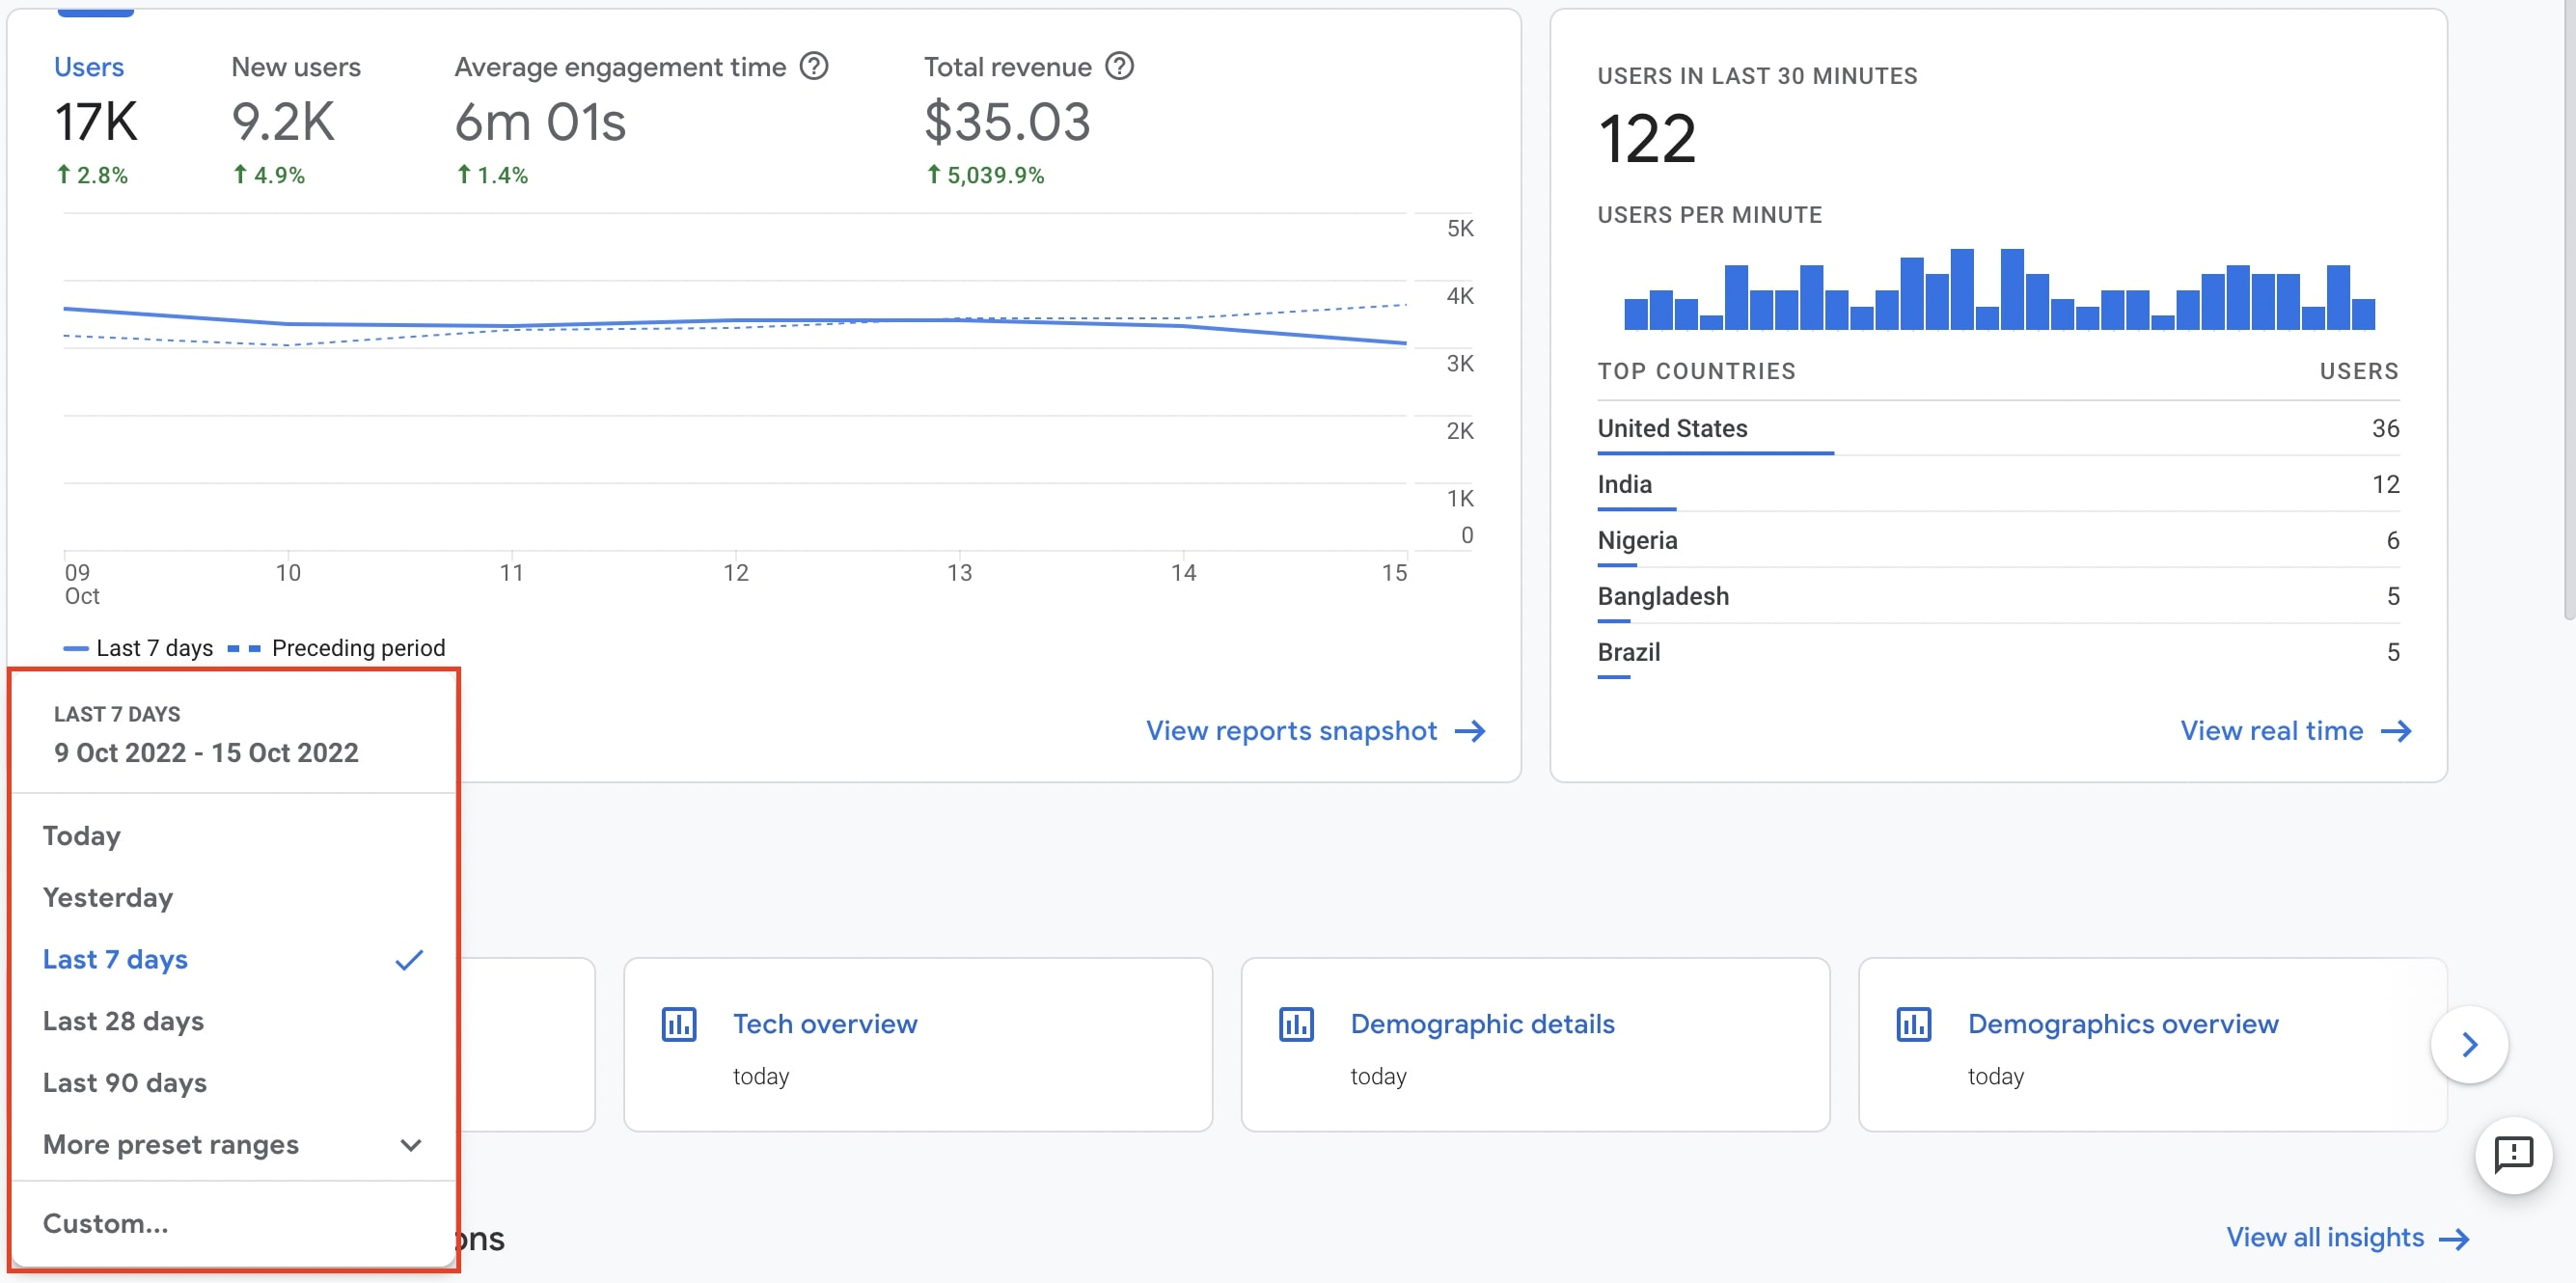
\includegraphics[width=1\textwidth]{problem-analysis/GA4-home}
    \caption{\acrshort{ga4} home dashboard.}\label{fig:GA4-dashboard}
\end{figure}

\begin{figure}[H]
    \centering
    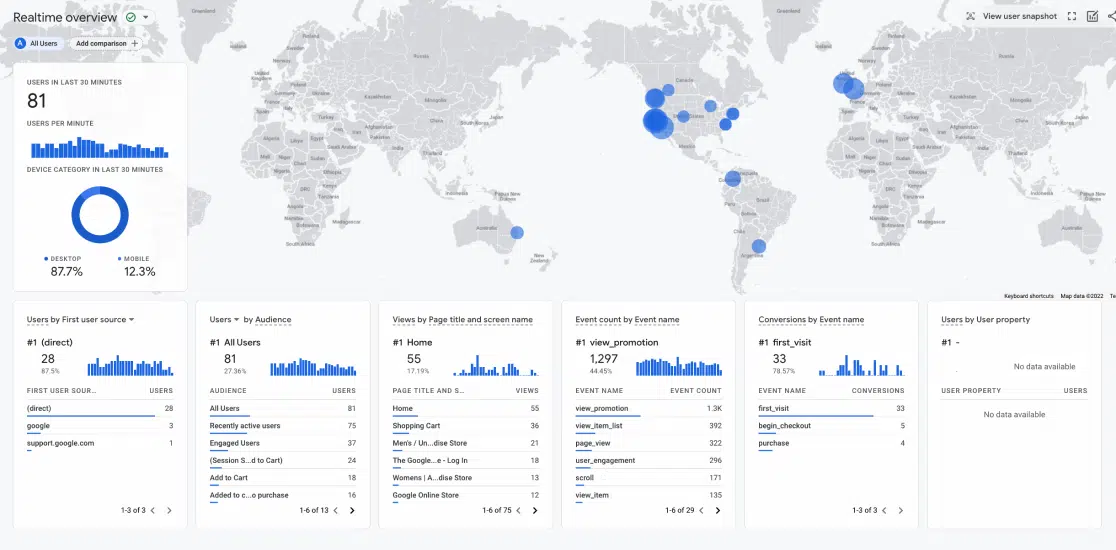
\includegraphics[width=1\textwidth]{problem-analysis/GA4-realtime}
    \caption{\acrshort{ga4} real-time page.}\label{fig:GA4-realtime}
\end{figure}
% textidote: ignore end

Figure~\ref{fig:GA4-dashboard} shows an example of the home dashboard in \acrshort{ga4}~\cite{ga4-interface}.
It is the first page the manager sees when logging in, and it provides an overview of the most important data.
The left side of the screen shows site activity in the last 7 days, but the graph can be changed to any time period.
The right side shows the number of users in the last 30 minutes, broken down to users per minute.
It's a very simple interface, but the power of \acrshort{ga4} lies deeper in the menus.

Figure~\ref{fig:GA4-realtime} shows an example of the real-time page in \acrshort{ga4}~\cite{ga4-realtime}.
This is a powerful tool that allows the manager to monitor the current activity of the site.
It shows a map with the locations of the users currently online and how they interact with the website.
This can be useful to monitor any changes caused by marketing campaigns, product launches or other events.

% textidote: ignore begin
\begin{figure}[H]
    \centering
    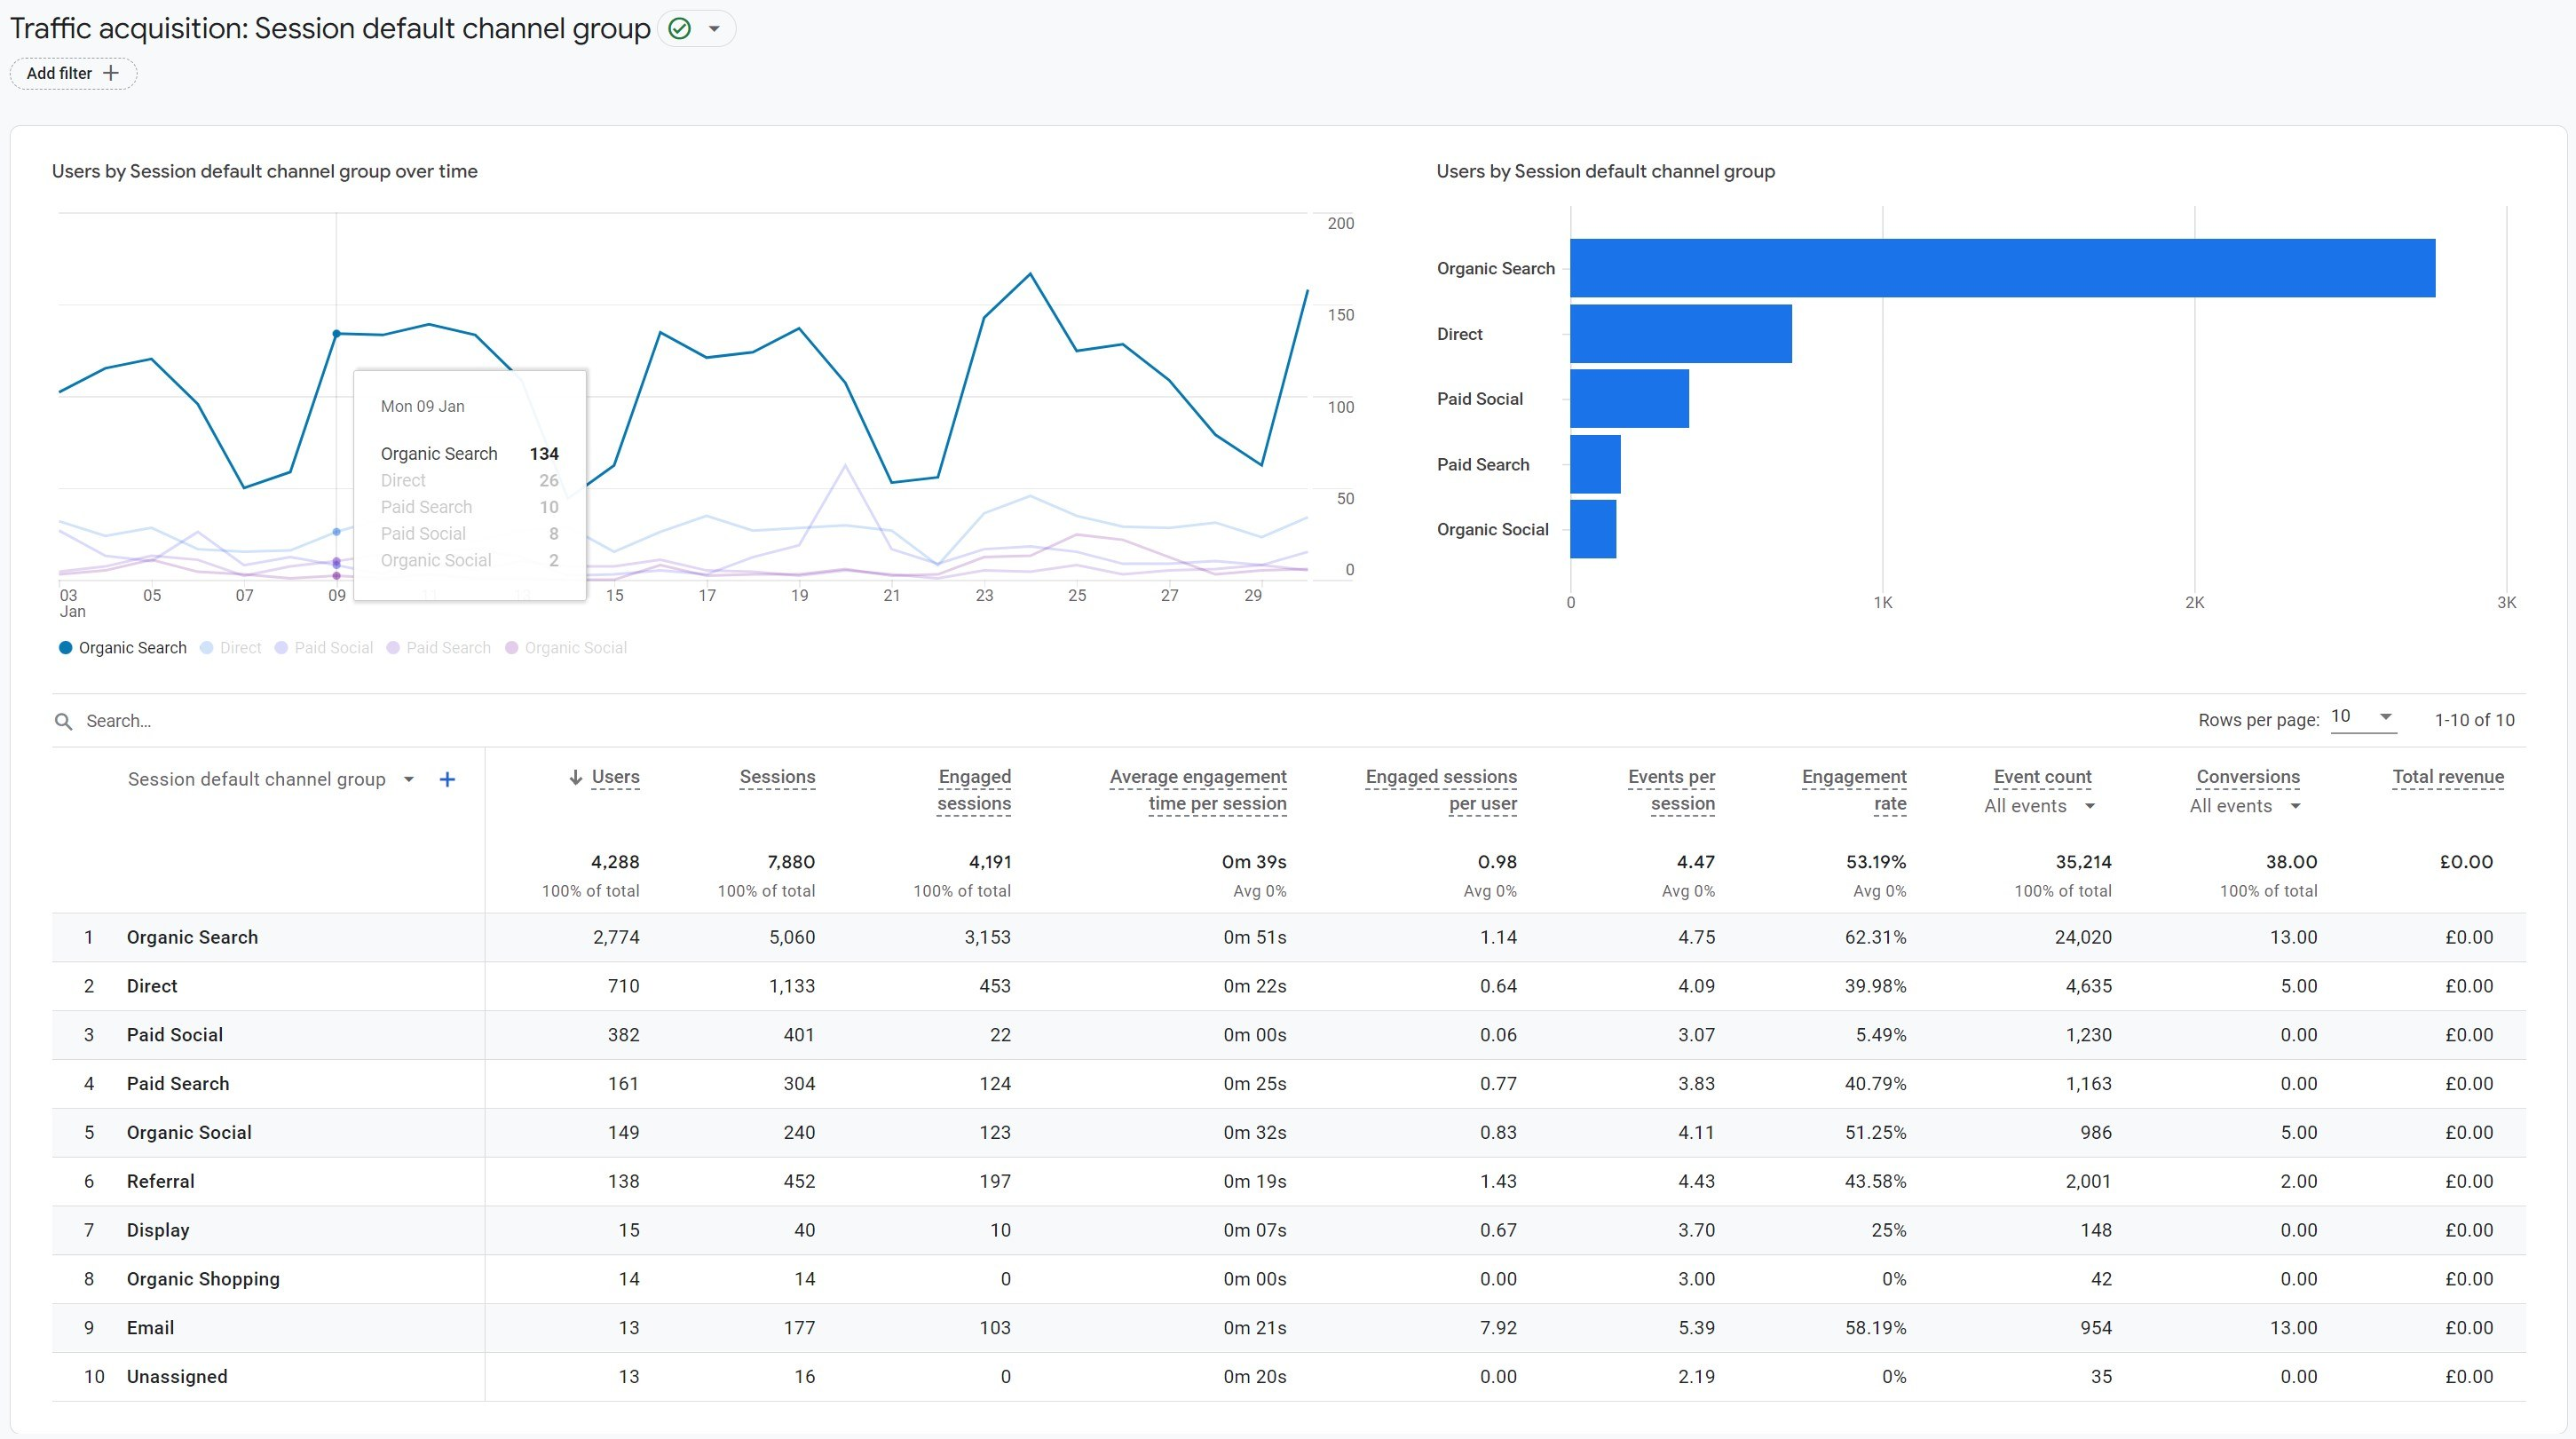
\includegraphics[width=1\textwidth]{problem-analysis/GA4-acquisition}
    \caption{\acrshort{ga4} session acquisition.}\label{fig:GA4-acquisition}
\end{figure}
% textidote: ignore end

Figure~\ref{fig:GA4-acquisition} shows an example of a session acquisition overview in \acrshort{ga4}~\cite{ga4-tips}.
This is one of the submenus in the dashboard, and it shows data on how users are acquired.
The top left graph show the number of users acquired each day per channel group and the top right graph shows the total
acquisition per channel group.
The list below breaks every channel group down into numbers, and it also shows user retention, engagement, and sales.
A channel group is a group of sources that a user can come from, such as organic search, direct link, paid
advertisement, and many more.
The main purpose of this overview is to show the manager if the marketing campaigns are effective and if the users are
then retained and engaged.

% textidote: ignore begin
\acrshort{ga4} has similar overviews for many other statistics that can be tracked, most notably being user engagement
and monetization.
% textidote: ignore end
User engagement shows how users interact with the website, such as how long they stay, how many pages they visit, and
how they navigate the site.
Monetization shows how the website makes money, such as how many products are sold, how much money is made, and how
many users are retained.

The disadvantages of \acrlong{ga4} are that it's limited in what services it can integrate with.
It is designed for digital services, so it can't natively track physical goods.
This means that \acrshort{ga4} cannot be utilized to solve the problem of tracking physical sales in a caf\'e.
The layout is also not very user-friendly, as it is designed for professionals, that are used to working with data.
It can however be customized to be more user-friendly, but it requires some work.
% textidote: ignore begin
\acrshort{ga4} is a free service, but it also offers a paid option, that allows for more features and better
support~\cite{ga4-360}.
% textidote: ignore end
